% PULib.tex -- The pileup library: the minimum-bias events of the Phase-2 mixing, before they are mixed.
% Chapter of the JitJet book (JitJetSW/Journey). Compile with
%     pdflatex PULib.tex && pdflatex PULib.tex
% from this directory; the figures are read from ../../test/PU_Phase2/ (runPileup_mcPhase2_BBbar.sh output).
% The mixing itself (MixingModule, CrossingFrames, the mixed pages) is the subject of PUSIM.tex.
\documentclass[11pt,a4paper]{article}

\usepackage[T1]{fontenc}
\usepackage[utf8]{inputenc}
\usepackage{lmodern}
\usepackage{textcomp}
\usepackage{microtype}
\usepackage[a4paper,margin=22mm,top=24mm,bottom=26mm]{geometry}
\usepackage{amsmath,amssymb}
\usepackage{graphicx}
\usepackage{xcolor}
\usepackage{booktabs}
\usepackage{multirow}
\usepackage{array}
\usepackage{tabularx}
\usepackage{longtable}
\usepackage{caption}
\usepackage{subcaption}
\usepackage{float}
\usepackage{placeins}
\usepackage{enumitem}
\usepackage{listings}
\usepackage{tikz}
\usetikzlibrary{arrows.meta,positioning,shapes.geometric,fit,calc}
\usepackage{fancyhdr}
\usepackage{url}
\urlstyle{tt}
\usepackage[colorlinks=true,linkcolor=blue!50!black,citecolor=blue!50!black,urlcolor=blue!50!black]{hyperref}

\graphicspath{{../../test/PU_Phase2/}}

% ---------------------------------------------------------------- colours (as in PUSIM.tex)
\definecolor{puearly}{RGB}{178,160,0}
\definecolor{puintime}{RGB}{102,153,255}
\definecolor{pulate}{RGB}{255,120,120}
\definecolor{sigchg}{RGB}{0,0,0}
\definecolor{signeu}{RGB}{153,0,153}
\definecolor{sigpho}{RGB}{0,153,0}
\definecolor{codebg}{RGB}{245,245,245}
\definecolor{histfill}{RGB}{84,116,168}     % one hue for all histograms of this chapter
\definecolor{histline}{RGB}{40,62,96}

\lstset{
  basicstyle=\ttfamily\footnotesize,
  backgroundcolor=\color{codebg},
  frame=single, framerule=0pt, framesep=4pt,
  breaklines=true, breakatwhitespace=false,
  columns=fullflexible, keepspaces=true,
  showstringspaces=false,
  xleftmargin=4pt, xrightmargin=4pt,
  aboveskip=6pt, belowskip=6pt,
}
\lstdefinestyle{py}{language=Python, keywordstyle=\color{blue!60!black}, commentstyle=\color{gray}, stringstyle=\color{green!40!black}}
\lstdefinestyle{sh}{language=bash, keywordstyle=\color{black}, commentstyle=\color{gray}}
\lstdefinestyle{cpp}{language=C++, keywordstyle=\color{blue!60!black}, commentstyle=\color{gray}}
\lstdefinestyle{txt}{language={}}

\newcommand{\code}[1]{\texttt{#1}}
\newcommand{\pt}{\ensuremath{p_{\mathrm{T}}}}
\newcommand{\bx}{\ensuremath{\mathrm{bx}}}
\newcommand{\bbbar}{\ensuremath{b\bar{b}}}
\newcommand{\GeV}{\,\mathrm{GeV}}
\newcommand{\MeV}{\,\mathrm{MeV}}
\newcommand{\TeV}{\,\mathrm{TeV}}
\newcommand{\ns}{\,\mathrm{ns}}
\newcommand{\ps}{\,\mathrm{ps}}
\newcommand{\cm}{\,\mathrm{cm}}
\newcommand{\mm}{\,\mathrm{mm}}
\newcommand{\um}{\,\mu\mathrm{m}}
\newcommand{\mb}{\,\mathrm{mb}}
\newcommand{\sigin}{\ensuremath{\sigma_{\mathrm{inel}}}}
\newcommand{\ptHat}{\ensuremath{\hat{p}_{\mathrm{T}}}}

% ---------------------------------------------------------------- "in plain words" boxes
\definecolor{plainbg}{RGB}{240,246,255}
\definecolor{plainrule}{RGB}{60,100,170}
\newsavebox{\plainbox}
\newenvironment{plainwords}[1][In plain words]{%
  \par\medskip\noindent\setlength{\fboxsep}{6pt}\setlength{\fboxrule}{0.6pt}%
  \begin{lrbox}{\plainbox}\begin{minipage}{\dimexpr\textwidth-2\fboxsep-2\fboxrule\relax}\small
  \textbf{\textcolor{plainrule}{#1.}}\ \ignorespaces}{%
  \end{minipage}\end{lrbox}\noindent\fcolorbox{plainrule}{plainbg}{\usebox{\plainbox}}\par\medskip}

\captionsetup{font=small,labelfont=bf,width=0.95\textwidth}
\setlist{nosep,leftmargin=*}
\emergencystretch=1.5em

\pagestyle{fancy}
\fancyhf{}
\fancyhead[L]{\small JitJet book -- The pileup library}
\fancyhead[R]{\small\thepage}
\renewcommand{\headrulewidth}{0.3pt}

\title{\textbf{The pileup library}\\[4pt]
  \large Fifty minimum-bias collisions for the Phase-2 mixing: how they are generated,\\
  what they contain, and what one of them looks like in the detector}
\author{JitJet book, \code{JitJetSW/Journey} -- \code{doc/pu/PULib.tex}}
\date{CMSSW\_15\_0\_5, Phase-2 detector D110, 14\,TeV; library of \code{test/PU\_Phase2/}, 26 October 2026}

\begin{document}
\maketitle

\begin{abstract}
\noindent
Before a signal event can be mixed with pileup, the pileup has to exist: a file of minimum-bias
proton--proton collisions, generated and simulated once, that the \code{MixingModule} will later overlay on
every signal event. This chapter is about that file and nothing else. It explains why a library of soft
collisions is the right raw material for pileup, which Pythia8 processes a minimum-bias event is made of and
with which cross sections, how the library of this book is produced with two \code{cmsDriver.py} steps (GEN
with the HL-LHC vertex smearing, SIM with the same Geant4 as the signal), why it needs its own random seeds,
what the GEN and GEN-SIM files contain product by product and byte by byte, and what the 50 events of the
library look like one by one: their process type, primaries, \code{SimTrack}s, hits and vertices, with the
statistics of the sample and the full page set of one event drawn with \code{SimHitAnalyzer} (case (b) of
the pileup chapter). It closes with the arithmetic of how large a library must be, where the production
libraries come from, and how to inspect, regenerate and enlarge the library with
\code{runPileup\_mcPhase2\_BBbar.sh}. The mixing itself -- the \code{MixingModule}, the \code{CrossingFrame}s
and the mixed pages -- is the subject of the companion chapter \code{PUSIM.tex}; everything here happens
before it. The chapter is written for a student who has followed the GEN and SIM chapters; the boxes marked
``In plain words'' restate each key idea without the CMSSW vocabulary.
\end{abstract}
\clearpage
\tableofcontents
\clearpage

% ======================================================================================================
\section{Before you start}
\label{sec:before}

\paragraph{What you should already know.} From the GEN chapter: that Pythia8 produces the particles of one
proton--proton collision, that a \emph{generator fragment} (a \code{\_cfi.py} file) tells it which process and
tune to use, and that \code{cmsDriver.py} writes a complete configuration from a few options. From the SIM
chapter: that Geant4 transports the stable particles (the \emph{primaries}) through the detector and leaves
\code{SimTrack}s, \code{SimVertex}s, \code{PSimHit}s (tracker, muon system, MTD) and \code{PCaloHit}s
(calorimeters) in the event, and how a \code{SimHitAnalyzer} page is read. Nothing about the mixing is
assumed; where the chapter needs to say what the library will be used for, it says it in one sentence and
points to \code{PUSIM.tex}.

\paragraph{Conventions.}
\begin{center}\small
\begin{tabularx}{\textwidth}{>{\raggedright\arraybackslash}p{40mm}X}
\toprule
word / symbol & meaning in this chapter \\
\midrule
library & a ROOT file of minimum-bias GEN-SIM events, made once and overlaid many times; here
  \code{step2\_SIM\_MinBias\_out.root}, 50 events \\
minimum bias & the inelastic proton--proton collisions in their natural proportions
  (Pythia8 \code{SoftQCD:inelastic}) \\
ND, SD, DD, CD & non-diffractive, single-, double- and central-diffractive collision (Pythia8 process codes
  101, 103/104, 105, 106) \\
stable particle & a particle with HepMC status 1 after Pythia8 has done its decays \\
primary & a stable particle handed to Geant4 (a \code{SimTrack} with a generator link); fewer than the
  stable particles because of the beam-pipe and momentum cuts of section~\ref{sec:simstep} \\
hit & one \code{PSimHit} or one \code{PCaloHit}; several hits can fall in the same calorimeter cell \\
PU, $\mu$ & the mean number of pileup collisions per bunch crossing of the scenario the library serves \\
event $k$ & the $k$-th event of the library file (run 1, lumi 1, event $k$); event 1 is the one drawn \\
case (b) & the pages of one library event alone, \code{PU\_Phase2/pileup/}, the naming of \code{PUSIM.tex} \\
\bottomrule
\end{tabularx}
\end{center}

\paragraph{Roadmap.} Section~\ref{sec:why} says what the library is for and what it must satisfy.
Section~\ref{sec:minbias} is about the physics of one minimum-bias event. Section~\ref{sec:making} follows the
two \code{cmsDriver.py} steps that make the library, option by option, including the vertex smearing and the
random seeds. Section~\ref{sec:content} opens the files: the products, their sizes, and a table of all 50
events with their statistics. Section~\ref{sec:oneevent} draws one event on the detector.
Section~\ref{sec:size} is the arithmetic of library sizes and a look at the production libraries, and
section~\ref{sec:extend} tells how to inspect, regenerate and extend the library.
Appendix~\ref{app:glossary} is a glossary.

% ======================================================================================================
\section{What the library is for}
\label{sec:why}

At the HL-LHC every bunch crossing (every $25\ns$) contains on average $\mu\simeq200$ inelastic
proton--proton collisions. One of them is the hard scattering the generator was asked for; the other
$\sim199$ are soft collisions that happen to occur in the same crossing, the \emph{pileup}, and the
collisions of the neighbouring crossings leak into the slow detectors too. A realistic simulated event is
therefore one signal event plus a Poisson-distributed number of soft collisions in each of several bunch
crossings: $7\times200 = 1400$ of them per signal event in the Phase-2 production window $\bx=-3\ldots+3$,
$3\times10=30$ in the exercise of this book.

\paragraph{The strategy.} CMSSW does not generate those 1400 collisions together with the signal. It
generates and simulates minimum-bias collisions \emph{once}, stores them in a file -- the \emph{pileup
library} -- and the \code{MixingModule} of the DIGI step later reads a random (here: sequential) selection
of them and adds their hits to the hits of the signal event before the digitisers run. The library is thus a
perfectly ordinary GEN-SIM sample whose only peculiarity is its purpose: its events are never looked at one
by one in an analysis, they are raw material to be stacked.

\begin{plainwords}[Why a library]
Geant4 is the expensive step of the chain (seconds per collision, section~\ref{sec:cost}), and the hits it
produces add up: a sensor crossed by two particles from two collisions holds two hits, a calorimeter cell
holds the sum of two energies. So nothing is lost by simulating each collision separately and adding the
hits afterwards, and a great deal is gained: one simulated minimum-bias collision can serve as pileup for
thousands of different signal events. The library is the stock of simulated collisions that makes this
possible.
\end{plainwords}

\paragraph{What a library must satisfy.} Because its events will be added to a signal event as if they
had happened in the same detector at the same moment, the library must be made under the same conditions
as the signal it will be mixed with:
\begin{enumerate}
\item \textbf{the same beam spot}: the vertex smearing runs in the GEN step, so each library event carries its
  vertex position \emph{and time} already; the mixing only adds the $25\ns\times\bx$ offset. A library made
  with a Run-3 beam spot would put its vertices in the wrong place for a Phase-2 signal
  (section~\ref{sec:vtx});
\item \textbf{the same geometry and the same Geant4 physics}: the hits must be of exactly the same nature
  (same sensitive volumes, same thresholds, same HF shower library) as the signal hits
  (section~\ref{sec:simstep});
\item \textbf{the same centre-of-mass energy}: $14\TeV$ for Phase-2;
\item \textbf{independent random numbers}: the library must not repeat the random sequence of the signal
  (section~\ref{sec:seeds});
\item \textbf{the products the mixing reads}: \code{SimTrack}s, \code{SimVertex}s, the \code{HepMCProduct},
  and every \code{PSimHit} and \code{PCaloHit} collection the digitisers consume (section~\ref{sec:products});
\item \textbf{enough events} for the pileup it has to provide (section~\ref{sec:size}).
\end{enumerate}
Points 1 to 3 are met by giving the two \code{cmsDriver.py} steps of the library the same \code{--conditions},
\code{--era}, \code{--geometry} and \code{--beamspot} as the signal; point 4 by explicit seeds; point 5 by the
\code{FEVTDEBUG} event content; point 6 by the \code{PUEVENTS} variable of the script.

% ======================================================================================================
\section{The minimum-bias event}
\label{sec:minbias}

\paragraph{Which collisions.} Pileup is made of the generic inelastic collisions, in their natural
proportions. In Pythia8 this is the process group \code{SoftQCD:inelastic}, the sum of four subprocesses:
\begin{center}\small
\begin{tabular}{llrrr}
\toprule
process & Pythia8 code & $\sigma$ [mb] & expected share & events of the 50 \\
\midrule
non-diffractive (ND), $pp\to X$ & 101 & 55.36 & 70.6\,\% & 35 \\
single diffractive (SD), $pp\to pX$ and $Xp$ & 103 + 104 & $2\times6.44$ & 16.4\,\% & 8 \\
double diffractive (DD), $pp\to XX$ & 105 & 8.88 & 11.3\,\% & 4 \\
central diffractive (CD), $pp\to pXp$ & 106 & 1.29 & 1.6\,\% & 3 \\
\midrule
inelastic, all & & 78.42 & 100\,\% & 50 \\
\bottomrule
\end{tabular}
\end{center}
{\sloppy The cross sections are those Pythia8 printed at the initialisation of the GEN step
(\code{step1\_GEN\_MinBias\_out.log}, ``PYTHIA Process Initialization''). They are not computed from the
PDFs: the CP5 tune fixes the total and the elastic cross sections, $\sigma_{\mathrm{tot}} = 100.309\mb$ and
$\sigma_{\mathrm{el}} = 21.89\mb$ (\code{SigmaTotal:mode = 0}), so that $\sigin = 78.42\mb$, and the
diffractive pieces are taken from Pythia's parametrisation; the non-diffractive part is what remains. The
\code{crossSection = 71.39e9} (pb) written in the fragment is older metadata that the \code{GenXsecAnalyzer}
reports at the end of the job (``total cross section $= 7.198\times10^{10}$ pb'': the 50 events of this
library were all accepted, 35 ND, 8 SD, 4 DD and 3 CD, as the table shows). With 50 events the observed
shares scatter around the expected ones by a few events, as they should.\par}

\begin{plainwords}[Soft, diffractive, minimum bias]
In a \emph{non-diffractive} collision the two protons break up completely; many soft particles come out,
mostly along the beam, and several parton pairs can interact in the same collision (multiple-parton
interactions, MPI), which is what makes the multiplicity so variable (section~\ref{sec:stats}). In a
\emph{diffractive} collision one proton (SD) or both (DD) survive intact or turn into a low-mass system, with
a large gap in rapidity in between: the central detector sees a few particles or nothing at all. In a
\emph{central-diffractive} collision both protons survive and a small system appears in the middle.
\emph{Minimum bias} is the historical name for a sample selected with the least possible trigger bias, i.e.\
essentially all inelastic collisions in their natural proportions. That is what pileup is made of, so the
library is a minimum-bias sample.
\end{plainwords}

\paragraph{The generator fragment.} The library uses the fragment that the Phase-2 RelVal and production
pileup libraries use, \path{Configuration/Generator/python/MinBias_14TeV_pythia8_TuneCP5_cfi.py}:
\begin{lstlisting}[style=py]
generator = cms.EDFilter("Pythia8ConcurrentGeneratorFilter",
    crossSection = cms.untracked.double(71.39e+09),   # pb, metadata only
    comEnergy = cms.double(14000.0),
    PythiaParameters = cms.PSet(
        pythia8CommonSettingsBlock,                      # what Pythia decays, error tolerance, LHAPDF preference
        pythia8CP5SettingsBlock,                         # the CP5 tune
        processParameters = cms.vstring('SoftQCD:inelastic = on'),
        parameterSets = cms.vstring('pythia8CommonSettings', 'pythia8CP5Settings', 'processParameters')))
\end{lstlisting}
Three blocks of Pythia8 settings go into it; the generated configuration
(\code{step1\_GEN\_MinBias\_cfg.py}) spells them out:
\begin{itemize}
\item \textbf{the process}: \code{SoftQCD:inelastic = on}, the four subprocesses above and nothing else (no
  hard QCD: a minimum-bias event with a $100\GeV$ jet is possible but comes from the tail of the MPI and
  shower, not from a $2\to2$ hard process);
\item \textbf{the tune CP5} (\code{Configuration/Generator/python/MCTunes2017/PythiaCP5Settings\_cfi.py}):
  \code{Tune:pp 14} (Monash as the starting point), the NNPDF3.1 NNLO PDF set with
  $\alpha_s(M_Z)=0.118$ at second order in the showers and in the MPI, the MPI regularisation
  \code{pT0Ref = 1.41} with its energy dependence \code{ecmPow = 0.03344}, the double-Gaussian proton
  profile (\code{bProfile = 2}, \code{coreRadius = 0.7634}, \code{coreFraction = 0.63}), the colour
  reconnection range 5.176, and the fixed $\sigma_{\mathrm{tot}}$ and $\sigma_{\mathrm{el}}$ quoted above.
  The tune is the same one the signal uses, so the underlying event of the signal and the pileup are
  described by the same model;
\item \textbf{the common settings} (\code{Pythia8CommonSettings\_cfi.py}): \code{ParticleDecays:limitTau0 = on}
  with \code{tau0Max = 10} (mm): Pythia decays every particle with $c\tau<10\mm$ ($\pi^0$, $\eta$, $D$ and
  $B$ hadrons, $\tau$, $\Sigma^0$, \ldots) and leaves the longer-lived ones ($K^0_S$ at $2.7\cm$,
  $\Lambda$ at $7.9\cm$, $K^\pm$, $\pi^\pm$, $\mu^\pm$, neutrons) to Geant4; this is why a
  \code{SimHitAnalyzer} page shows a $\Lambda$ or a $K^0_S$ as a primary and never a $\pi^0$.
\end{itemize}

\paragraph{What one event looks like at the generator level.} The 50 events of the library have between 4
and 716 stable particles (mean 174, median 106), of which between 0 and 118 are ``central'' ($|\eta|<2.5$,
$\pt>0.5\GeV$, what the tracker will see; mean 19, median 8). The hardest stable particle of an event has
$\pt$ between $0.3$ and $9.7\GeV$ (mean $2.3\GeV$), and the scalar sum of $\pt$ over the whole event is
$0.7$ to $389\GeV$. These are soft events: the signal \bbbar{} event of the book has $\ptHat>100\GeV$ in a
single parton pair. The multiplicity is driven by the process type and, within the non-diffractive class,
by the number of MPI: section~\ref{sec:stats} gives the per-process means.

% ======================================================================================================
\section{Making the library}
\label{sec:making}

The script \code{runPileup\_mcPhase2\_BBbar.sh} makes the library with two \code{cmsDriver.py} calls, with
the Run4D110 RelVal settings of the signal (\code{runCMSDrivers\_mcPhase2\_BBbar\_SIM.sh}):
\begin{lstlisting}[style=sh]
# step 1, GEN: 50 minimum-bias events, HL-LHC vertex smearing, own random seeds
cmsDriver.py MinBias_14TeV_pythia8_TuneCP5_cfi --conditions auto:phase2_realistic_T33 --era Phase2C17I13M9 \
  --geometry ExtendedRun4D110 --beamspot DBrealisticHLLHC -n 50 -s GEN --datatier GEN --eventcontent FEVTDEBUG \
  --fileout file:step1_GEN_MinBias_out.root --python_filename step1_GEN_MinBias_cfg.py --no_exec \
  --customise_commands "process.RandomNumberGeneratorService.generator.initialSeed = 20261\nprocess.RandomNumberGeneratorService.VtxSmeared.initialSeed = 20262"
cmsRun step1_GEN_MinBias_cfg.py > step1_GEN_MinBias_out.log 2>&1
# step 2, SIM: the same Geant4 as the signal
cmsDriver.py step2 --filein file:step1_GEN_MinBias_out.root --conditions auto:phase2_realistic_T33 --era Phase2C17I13M9 \
  --geometry ExtendedRun4D110 --beamspot DBrealisticHLLHC -n -1 -s SIM --datatier GEN-SIM --eventcontent FEVTDEBUG \
  --fileout file:step2_SIM_MinBias_out.root --python_filename step2_SIM_MinBias_cfg.py --no_exec \
  --customise_commands "process.RandomNumberGeneratorService.g4SimHits.initialSeed = 20263"
cmsRun step2_SIM_MinBias_cfg.py > step2_SIM_MinBias_out.log 2>&1
\end{lstlisting}
Figure~\ref{fig:flow} shows the two steps and their files; the companion chapter takes over at the arrow
that leaves the figure.

\begin{figure}[H]
\centering
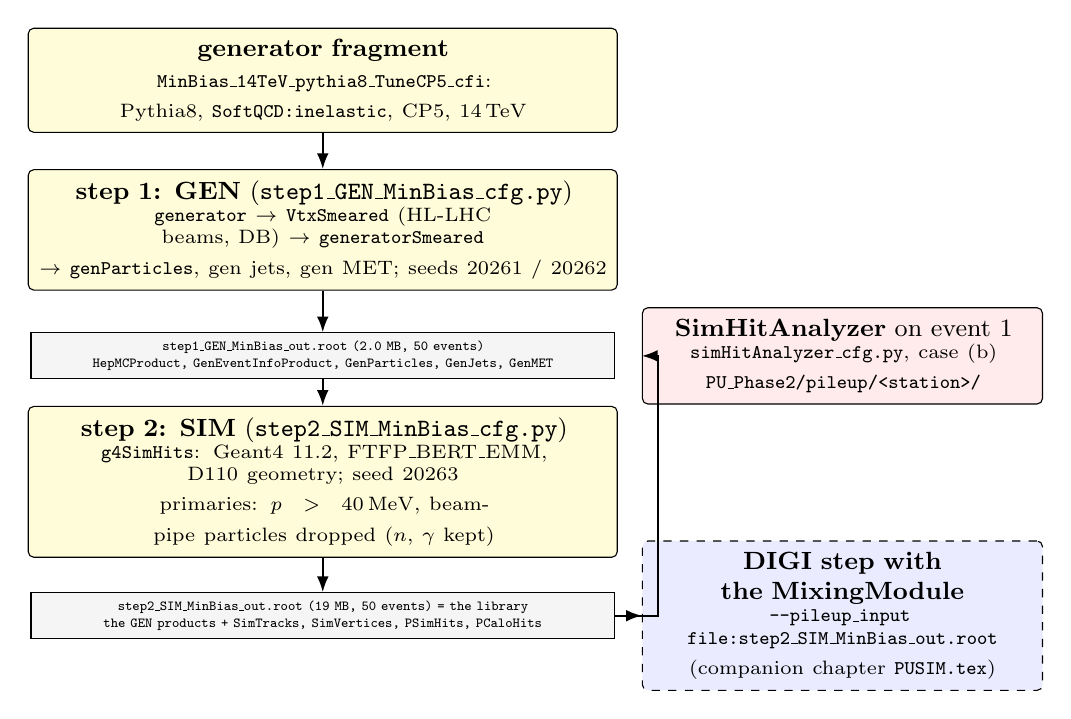
\begin{tikzpicture}[
  box/.style={draw, rounded corners=2pt, align=center, font=\small, minimum height=8mm, inner sep=4pt, fill=white},
  file/.style={draw, align=center, font=\tiny\ttfamily, inner sep=3pt, fill=gray!8},
  arr/.style={-{Latex[length=2mm]}, thick},
  lab/.style={font=\scriptsize, text=gray!60!black, fill=white, inner sep=1pt},
]
\node[box, fill=yellow!15, text width=72mm] (frag) at (0,0) {\textbf{generator fragment}\\\scriptsize \code{MinBias\_14TeV\_pythia8\_TuneCP5\_cfi}: Pythia8, \code{SoftQCD:inelastic}, CP5, 14\,TeV};
\node[box, fill=yellow!15, text width=72mm] (gen) at (0,-1.9) {\textbf{step 1: GEN} (\code{step1\_GEN\_MinBias\_cfg.py})\\\scriptsize \code{generator} $\to$ \code{VtxSmeared} (HL-LHC beams, DB) $\to$ \code{generatorSmeared}\\\scriptsize $\to$ \code{genParticles}, gen jets, gen MET; seeds 20261 / 20262};
\node[file, text width=72mm] (gfile) at (0,-3.5) {step1\_GEN\_MinBias\_out.root (2.0 MB, 50 events)\\HepMCProduct, GenEventInfoProduct, GenParticles, GenJets, GenMET};
\node[box, fill=yellow!15, text width=72mm] (sim) at (0,-5.1) {\textbf{step 2: SIM} (\code{step2\_SIM\_MinBias\_cfg.py})\\\scriptsize \code{g4SimHits}: Geant4 11.2, FTFP\_BERT\_EMM, D110 geometry; seed 20263\\\scriptsize primaries: $p>40\MeV$, beam-pipe particles dropped ($n$, $\gamma$ kept)};
\node[file, text width=72mm] (sfile) at (0,-6.8) {step2\_SIM\_MinBias\_out.root (19 MB, 50 events) = the library\\the GEN products + SimTracks, SimVertices, PSimHits, PCaloHits};
\node[box, fill=blue!8, text width=48mm, dashed] (mix) at (6.6,-6.8) {\textbf{DIGI step with the MixingModule}\\\scriptsize \code{--pileup\_input file:step2\_SIM\_MinBias\_out.root}\\\scriptsize (companion chapter \code{PUSIM.tex})};
\node[box, fill=red!8, text width=48mm] (ana) at (6.6,-3.5) {\textbf{SimHitAnalyzer} on event 1\\\scriptsize \code{simHitAnalyzer\_cfg.py}, case (b)\\\scriptsize \code{PU\_Phase2/pileup/<station>/}};
\draw[arr] (frag) -- (gen); \draw[arr] (gen) -- (gfile); \draw[arr] (gfile) -- (sim); \draw[arr] (sim) -- (sfile);
\draw[arr, dashed] (sfile) -- (mix);
\draw[arr] (sfile.east) -- ++(0.55,0) |- (ana.west);
\end{tikzpicture}
\caption{The two steps that make the library and the two consumers of the result: the analyzer that draws
one of its events (section~\ref{sec:oneevent}) and, outside this chapter, the mixing job.}
\label{fig:flow}
\end{figure}

\subsection{The \code{cmsDriver.py} options}

For a reader who has not written a \code{cmsDriver.py} command before: it is the tool that writes a
complete CMSSW configuration (a \code{\_cfg.py} file) from a few options and then, unless \code{--no\_exec}
is given, runs it. The options of the two library steps:
\begin{center}\small
\begin{tabularx}{\textwidth}{>{\raggedright\arraybackslash}p{54mm}X}
\toprule
option & what it sets \\
\midrule
first argument (\code{MinBias\_14TeV\_\ldots\_cfi}, \code{step2}) & the generator fragment to load (GEN step),
  or just a name for the configuration (SIM step) \\
\code{-s GEN}, \code{-s SIM} & the step to run: the generator sequence \code{pgen}, or the Geant4 sequence
  \code{psim} \\
\code{--filein}, \code{--fileout} & input and output ROOT files; the GEN step has no input
  (\code{EmptySource}) \\
\code{-n 50}, \code{-n -1} & number of events to generate ($-1$ in the SIM step: all events of the input) \\
\code{--conditions auto:phase2\_realistic\_T33} & the global tag: alignment, calibrations, the HL-LHC beam-spot
  payload (section~\ref{sec:vtx}), \ldots \\
\code{--era Phase2C17I13M9} & the set of era modifiers that adapt every module to the Phase-2 detector \\
\code{--geometry ExtendedRun4D110} & the detector geometry Geant4 is built from (D110, the current Phase-2
  layout) \\
\code{--beamspot DBrealisticHLLHC} & the vertex-smearing module of the GEN step: \code{HLLHCEvtVtxGenerator}
  with parameters from the database \\
\code{--datatier GEN}, \code{GEN-SIM}; \code{--eventcontent FEVTDEBUG} & how the output is labelled and which
  products it keeps (\code{FEVTDEBUG}: everything, including every SimHit collection) \\
\code{--customise\_commands "..."} & Python lines appended verbatim to the end of the configuration (a literal
  \code{\textbackslash n} separates lines); here the seeds \\
\code{--python\_filename}, \code{--no\_exec} & the name of the configuration, and ``write it, do not run it''
  (the script runs \code{cmsRun} itself so that it can keep the log) \\
\bottomrule
\end{tabularx}
\end{center}

\subsection{Step 1: the GEN step}
\label{sec:genstep}

The generated configuration is a process named \code{GEN} with the era \code{Phase2C17I13M9}. Its schedule
has one path and three end paths:
\begin{lstlisting}[style=py]
process.generation_step = cms.Path(process.pgen)               # the generator sequence
process.genfiltersummary_step = cms.EndPath(process.genFilterSummary)
process.endjob_step = cms.EndPath(process.endOfProcess)
process.FEVTDEBUGoutput_step = cms.EndPath(process.FEVTDEBUGoutput)
process.schedule = cms.Schedule(process.generation_step, process.genfiltersummary_step, process.endjob_step, process.FEVTDEBUGoutput_step)
for path in process.paths:
    getattr(process, path).insert(0, process.ProductionFilterSequence)   # the generator filter runs first in every path
\end{lstlisting}
and \code{pgen} (\code{Configuration/StandardSequences/python/Generator\_cff.py}) is
\begin{lstlisting}[style=py]
pgen = cms.Sequence(randomEngineStateProducer + VertexSmearing + GenSmeared + GeneInfo + genJetMET, PPSTransportTask)
\end{lstlisting}
Module by module, for every event:
\begin{enumerate}
\item \code{generator} (\code{Pythia8ConcurrentGeneratorFilter}) runs Pythia8 and puts the event as a
  \code{HepMCProduct} labelled \code{generator:unsmeared} into the event, with the vertex at the origin, plus a
  \code{GenEventInfoProduct} (process id, weights, $\hat{p}_{\mathrm{T}}$ of the hardest interaction). It is a
  \emph{filter}: a fragment can reject events (a \bbbar{} filter, a $\ptHat$ cut); this fragment accepts
  everything (\code{filterEfficiency = 1.0}, and the \code{GenXsecAnalyzer} of the log confirms 50/50);
\item \code{randomEngineStateProducer} records the state of every random engine at the start of the event
  (\code{edm::RandomEngineStates}), so that any single event can be reproduced later;
\item \code{VtxSmeared} (\code{HLLHCEvtVtxGenerator}) moves the whole event to a vertex drawn from the beam
  model, in space and in time, and writes the moved copy as \code{generatorSmeared} (section~\ref{sec:vtx});
\item \code{genParticles} converts the HepMC record into \code{reco::GenParticle}s, with the vertex
  (\code{genParticles:xyz0}) and time (\code{genParticles:t0}) of the event; \code{genJetMET} clusters the
  generator jets (\code{ak4GenJets}, \code{ak8GenJets}, with and without neutrinos) and the generator MET.
  These are not used by the mixing; they are in the file because the standard GEN sequence makes them.
\end{enumerate}
The output module writes every product (\code{FEVTDEBUG}) of the events that passed the generation path.

\begin{plainwords}[Modules, products and the schedule]
A CMSSW job is a set of \emph{modules} (producers that add products to the event, filters that can stop the
processing of an event, analyzers that only read, output modules that write) and a \emph{schedule} that says
in which order they run for every event. A \code{Path} is an ordered list of modules; an \code{EndPath} runs
after all paths and is where the output modules go. Every product is identified by its type, the module that
made it, an optional instance label and the process name: ``\code{edm::HepMCProduct generatorSmeared
GEN}'' is the smeared HepMC event made by the module \code{generatorSmeared} in the process \code{GEN}.
\code{edmDumpEventContent file.root} lists them (section~\ref{sec:products}).
\end{plainwords}

\subsection{The vertex smearing}
\label{sec:vtx}

Pythia8 puts every collision at the origin. The real collisions are spread over the \emph{luminous region},
the overlap of the two bunches, and this is what \code{VtxSmeared} reproduces. For the HL-LHC the module
is the \code{HLLHCEvtVtxGenerator} (\code{IOMC/EventVertexGenerators}), which does not draw from a simple
Gaussian but from the density of two crossing, crab-rotated bunches:
\begin{lstlisting}[style=py]
# IOMC/EventVertexGenerators/python/VtxSmearedRealisticHLLHC_cfi.py  (--beamspot DBrealisticHLLHC)
from IOMC.EventVertexGenerators.HLLHCEvtVtxGenerator_cfi import HLLHCEvtVtxGenerator
VtxSmeared = HLLHCEvtVtxGenerator.clone(src = "generator:unsmeared", readDB = True)
\end{lstlisting}
With \code{readDB = True} the beam parameters come from the \code{SimBeamSpotHLLHCObjectsRcd} payload of the
global tag; the parameters of the model (and their nominal HL-LHC values of the non-DB configuration
\code{VtxSmearedHLLHC\_cfi}) are:
\begin{center}\small
\begin{tabularx}{\textwidth}{>{\raggedright\arraybackslash}p{66mm}Xr}
\toprule
parameter & meaning & nominal \\
\midrule
\code{EprotonInGeV} & beam energy & 7000 \\
\code{CrossingAngleInurad} & full crossing angle of the beams & 510 \\
\code{CrabbingAngleCrossingInurad}, \code{CrabFrequencyInMHz} & crab-cavity rotation of the bunches and the RF
  frequency of the cavities & 380, 400 \\
\code{BetaCrossingPlaneInm}, \code{BetaSeparationPlaneInm} & $\beta^\ast$ in the two planes & 0.20, 0.20 \\
\code{HorizontalEmittance}, \code{VerticalEmittance} & normalised emittances [m] & $2.5$, $2.05\times10^{-6}$ \\
\code{BunchLengthInm} & r.m.s.\ length of one bunch & 0.090 \\
\code{MeanXIncm}, \code{MeanYIncm}, \code{MeanZIncm}, \code{TimeOffsetInns} & the centre of the luminous
  region in space and time & 0 \\
\bottomrule
\end{tabularx}
\end{center}
The module samples $(x, y, z, t)$ from the product of the two bunch densities (an accept--reject loop on the
analytic intensity $I(x,y,z,t)$ of the crossing bunches, including the crab rotation), and shifts every
vertex of the HepMC event by that four-vector. Two consequences are worth remembering:
\begin{itemize}
\item \textbf{the spread along $z$ comes from the bunch length}: two $9\cm$ long bunches pass through
  each other, a collision can happen anywhere in the overlap, and the result is a near-Gaussian with
  $\sigma_z\simeq4.3\cm$ (the crossing angle and the crab cavities shorten it from the
  $9/\sqrt{2}\simeq6.4\cm$ that head-on bunches would give);
\item \textbf{the spread in time comes from the same overlap}: the overlap lasts a fraction of a nanosecond,
  $\sigma_t\simeq190\ps$. This time is \emph{part of the library event}: Geant4 starts every particle at the
  smeared vertex time, so every hit of the library already carries it, and the timing detectors (MTD, HGCal)
  will see library events arriving a few hundred picoseconds before or after the signal.
\end{itemize}
In the 50 events of this library the vertices have (sample r.m.s.) $\sigma_x = 9.6\um$,
$\sigma_y = 5.5\um$, $\sigma_z = 4.4\cm$ and $\sigma_t = 164\ps$, with $z$ from $-11.1$ to $+15.1\cm$ and $t$
from $-0.30$ to $+0.30\ns$ (table~\ref{tab:events}, figure~\ref{fig:hist}): consistent with the nominal
widths within the statistics of 50 events. The transverse size is microns, far below anything the pages
show; the longitudinal and time spreads are the ones that matter, because they are what the vertex finder
and the timing detectors will later use to separate the pileup collisions from the signal.

\begin{plainwords}[The same smearing as the signal, on purpose]
The signal \bbbar{} event of the book was generated with the very same \code{VtxSmeared} module. When the
library is later mixed into it, the library vertices are \emph{not} smeared again: the mixing takes each
library event as it is, vertex time included, and only adds the bunch-crossing offset. So the library has to
be made with the beam spot of the scenario it will serve. A library made with the Run-3 beam spot
($\sigma_z\simeq3.5\cm$, no time spread beyond what the bunches give) mixed into a Phase-2 signal would
simply be wrong, and nothing in the mixing job would notice.
\end{plainwords}

\subsection{Random seeds}
\label{sec:seeds}

The random numbers of a CMSSW job are pseudo-random: every module that needs them has its own engine in the
\code{RandomNumberGeneratorService}, and a given \code{initialSeed} always produces the same sequence. This is
what makes every job reproducible, and it is also a trap: \code{cmsDriver.py} writes the \emph{same default
seeds} into every configuration it generates. Had the library been made with the defaults, its GEN step would
have drawn the same vertex-smearing sequence as the signal's GEN step: library event $k$ would have had
\emph{exactly} the vertex of signal event $k$, and the first mixed pileup event would have sat on top of the
signal vertex, in space and in time. The script therefore sets, from its \code{PUSEED} variable (default
20261):
\begin{center}\small
\begin{tabular}{lll}
\toprule
engine & seed & what it drives \\
\midrule
\code{generator} & \code{PUSEED} $=20261$ & Pythia8: which process, MPI, showers, hadronisation, decays \\
\code{VtxSmeared} & \code{PUSEED}$+1 = 20262$ & the vertex position and time of every event \\
\code{g4SimHits} & \code{PUSEED}$+2 = 20263$ & Geant4: every interaction, shower and decay in the detector \\
\bottomrule
\end{tabular}
\end{center}
A different \code{PUSEED} gives a different library (different events, different vertices); the same
\code{PUSEED} always gives this one. The \code{randomEngineStateProducer} product of every event records the
engine states, so that a single event can be reproduced without regenerating the ones before it.

\subsection{Step 2: the SIM step}
\label{sec:simstep}

The SIM configuration loads \code{SimIdeal\_cff} and runs the standard full-physics Geant4 step
(\code{g4SimHits}, Geant4 11.2 in multi-threaded mode, physics list \code{FTFP\_BERT\_EMM}, the stage
\code{Transport\_B\_Decay\_EM\_Had} of the SIM chapter) on the D110 geometry: exactly what the signal went
through. What \code{g4SimHits} does with a library event:
\begin{enumerate}
\item it reads the smeared HepMC event (\code{generatorSmeared}) and converts the stable particles into
  Geant4 primaries, applying the cuts of the \code{Generator} block of \code{g4SimHits\_cfi}
  (\code{SimG4Core/Generators/src/Generator.cc}): a particle that would fly down the beam pipe (it reaches
  the far end of the vacuum chamber inside the pipe radius, i.e.\ $|\eta|$ beyond $\sim5.5$) is dropped
  unless it is a neutron or a photon, which are kept for the ZDC; every other particle must have
  $p>40\MeV$ (\code{MinPCut}) and $|\eta|<5.5$ (\code{MaxEtaCut}). The beam remnants and the surviving
  protons of the diffractive events are dropped here: this is why the number of \emph{primaries handed to
  Geant4} is smaller than the number of stable particles (182 of 215 for event 1, 1 of 11 for the
  central-diffractive event 5, 1 of 4 for the single-diffractive event 47; table~\ref{tab:events}). The one
  primary of event 47 is a $186\GeV$ photon at $\eta=9.1$, inside the beam pipe, that never meets a
  sensitive volume; the one of event 5 is a $1.9\GeV$ photon at $\eta=4.3$ that leaves nothing in the HF;
\item it transports them, with the secondaries they produce, through the detector and leaves one
  \code{SimTrack} per particle it decided to keep (every primary; secondaries above the saving thresholds),
  one \code{SimVertex} per interaction or decay point, and the hits: \code{PSimHit}s in the tracker, the muon
  chambers and the MTD, \code{PCaloHit}s in every calorimeter cell crossed;
\item every \code{SimTrack} of a primary keeps its link to the generator particle (\code{genpartIndex()}),
  which is how \code{SimHitAnalyzer} counts the primaries and traces every hit to one of them.
\end{enumerate}
The output keeps the GEN products untouched and adds the SIM products (\code{FEVTDEBUG}, next section).

\subsection{Cost: time and size}
\label{sec:cost}

From the timestamps of the two logs:
\begin{center}\footnotesize
\begin{tabular}{lllll}
\toprule
step & initialisation & event loop (50 events) & per event & output \\
\midrule
GEN & $\sim$1 min (Pythia MPI tables, LHAPDF) & 1.2\,s & 24\,ms & 2.0\,MB, 41\,kB/event \\
SIM & $\sim$80\,s (geometry, physics tables) & 178\,s & 3.6\,s mean & 19\,MB, 380\,kB/event \\
\bottomrule
\end{tabular}
\end{center}
The Geant4 time is proportional to the number of primaries: from 2\,ms for the one-photon events 5 and 47 to
14\,s for event 7 (498 primaries) and 24\,s for event 25 (633 primaries), i.e.\ $\sim30$\,ms per primary. A
minimum-bias event costs on average $3.6$\,s against $\sim4$\,s for a signal event of the book; the library is
cheap per event, but a production library is large (section~\ref{sec:size}), and the SIM step is where all of
its cost is.

% ======================================================================================================
\section{What is in the library}
\label{sec:content}

\subsection{The products}
\label{sec:products}

\code{edmDumpEventContent step2\_SIM\_MinBias\_out.root} lists what every event of the library holds. Grouped
by what the mixing will do with them:
\begin{center}\small
\begin{tabularx}{\textwidth}{>{\raggedright\arraybackslash\hyphenpenalty=10000}p{70mm}X}
\toprule
product (type, module:label) & role \\
\midrule
\multicolumn{2}{l}{\emph{read by the mixing (the \code{mixObjects} of the \code{MixingModule})}} \\
\code{vector<SimTrack> g4SimHits}, \code{vector<SimVertex> g4SimHits} & the particles and vertices of the
  event; the truth of every mixed hit \\
\code{edm::HepMCProduct generatorSmeared} & the generator record with the smeared vertex (\code{mixHepMC}) \\
\code{vector<PSimHit> g4SimHits:TrackerHits\ldots{}LowTof}, \code{\ldots{}HighTof} (\code{PixelBarrel}, \code{PixelEndcap}, \code{TIB}, \code{TID}, \code{TOB}, \code{TEC}) & the tracker hits; in the
  Phase-2 layout the inner tracker fills \code{PixelBarrel} / \code{PixelEndcap} and the outer tracker
  \code{TOB} / \code{TID}; \code{TIB} and \code{TEC} are empty \\
\code{vector<PSimHit> g4SimHits:MuonDTHits}, \code{MuonCSCHits}, \code{MuonRPCHits}, \code{MuonGEMHits}, \code{MuonME0Hits} & the muon-chamber hits \\
\code{vector<PSimHit> g4SimHits:FastTimerHitsBarrel}, \code{FastTimerHitsEndcap} & the MTD hits \\
\code{vector<PCaloHit> g4SimHits:EcalHitsEB} & the EB crystals (no \code{EcalHitsEE} / \code{ES} in Phase-2:
  both are empty) \\
\code{vector<PCaloHit> g4SimHits:HcalHits} & HB, HO and HF (the HF energies in shower-library units) \\
\code{vector<PCaloHit> g4SimHits:HGCHitsEE}, \code{HGCHitsHEfront}, \code{HGCHitsHEback} & the three HGCal sections (added to
  \code{mixCH} by the \code{phase2\_hgcal} era modifier) \\
\code{vector<PCaloHit> g4SimHits:ZDCHITS}, \code{CastorFI} & forward detectors, mixed but empty here \\
\midrule
\multicolumn{2}{l}{\emph{carried along, not mixed}} \\
\code{GenEventInfoProduct generator}; \code{vector<reco::GenParticle> genParticles} (+ \code{xyz0}, \code{t0}); \code{ak4GenJets}, \code{ak8GenJets}, \code{genMetTrue}, \ldots & the generator-level view of the
  event: useful to inspect the library (process id, vertex, multiplicity), ignored by the mixing \\
\code{vector<PCaloHit> g4SimHits:CalibrationHGCHits\ldots}, \code{CaloHitsTk}, \code{HFNoseHits}; \code{vector<PSimHit> g4SimHits:BCM1FHits}, \code{PLTHits}, \code{BHMHits}, \code{CTPPS\ldots{}Hits} & auxiliary
  and forward collections kept by \code{FEVTDEBUG}, empty or unused here \\
\code{edm::RandomEngineStates randomEngineStateProducer} (GEN and SIM), \code{edm::TriggerResults} & the
  engine states at the start of every event, and the result of the generator filter \\
\bottomrule
\end{tabularx}
\end{center}
A library needs the first group; a production library made with a leaner event content would drop the
second. The size of the file is dominated by the SIM products: per event, after compression,
\code{edmEventSize -v} reports $\sim94$\,kB of \code{SimTrack}s, $69$\,kB of EB hits, $63$ and $36$\,kB of
inner-tracker endcap and barrel hits, $26$\,kB of HepMC, $25$\,kB of HGCal EE hits and $20$\,kB of
\code{SimVertex}s, i.e.\ $\sim380$\,kB in all. The \code{SimTrack}s weigh more than any hit collection: a
minimum-bias event has on average $1000$ of them (table~\ref{tab:stats}), most of them shower secondaries
in the calorimeters.

\begin{plainwords}[GEN, GEN-SIM, and why the SimTracks are heavy]
The GEN file holds only what Pythia8 made (41\,kB per event). The GEN-SIM file holds that plus everything
Geant4 made (380\,kB per event): every stored particle of every shower as a \code{SimTrack}, and every hit.
When the mixing reads a library event it reads all of it, so the per-event size of the library is what sets
the input rate of a mixing job: at $\mathrm{PU}=200$ in seven crossings, $1400\times380\,\mathrm{kB}
\simeq 0.5$\,GB per signal event.
\end{plainwords}

\subsection{The 50 events}
\label{sec:events}

Table~\ref{tab:events} is the catalogue of the library: every event with its process type, its generator
multiplicity, what Geant4 made of it, and where and when its vertex is. The numbers are read from the two
files with the FWLite script of section~\ref{sec:inspect}. The first 18 rows are, in this order, the events
that the mixing job of the companion chapter put into the bunch crossings $-1$ (events 1--7), $0$ (8--15)
and $+1$ (16--18) of signal event 1; its table of mixed events is this table with the first 18 rows and the
$25\ns\times\bx$ offset added to $t$.

\begingroup
\scriptsize
\setlength{\tabcolsep}{2pt}
\renewcommand{\arraystretch}{1.02}
\begin{longtable}{rlrrrrrrrrrrr}
\caption{The 50 events of the library (\code{step1\_GEN\_MinBias\_out.root}, \code{step2\_SIM\_MinBias\_out.root}).
Process: Pythia8 subprocess (ND non-diffractive, SD single, DD double, CD central diffractive). Stable: HepMC
status-1 particles; primaries: \code{SimTrack}s with a generator link, i.e.\ the stable particles that
Geant4 received (above $40\MeV$ and not lost down the beam pipe, section~\ref{sec:simstep}). Tracker hits: all inner- and outer-tracker
\code{PSimHit}s; EB, HGCal (EE + HSi + HSc) and HCAL (HB + HO + HF) hits: \code{PCaloHit}s, several per
cell. $E_{\mathrm{EB}}$: summed EB \code{PCaloHit} energy. $z$ and $t$: the smeared primary vertex. Event 1 is
the one drawn in section~\ref{sec:oneevent}; events 1--18 are the ones mixed in the companion chapter.}
\label{tab:events}\\
\toprule
event & proc. & stable & prim. & SimTrk & SimVtx & TRK hits & EB hits & HGCal hits & HCAL hits & $E_{\mathrm{EB}}$ [GeV] & $z$ [cm] & $t$ [ns] \\
\midrule
\endfirsthead
\toprule
event & proc. & stable & prim. & SimTrk & SimVtx & TRK hits & EB hits & HGCal hits & HCAL hits & $E_{\mathrm{EB}}$ [GeV] & $z$ [cm] & $t$ [ns] \\
\midrule
\endhead
\midrule \multicolumn{13}{r}{\emph{continued on the next page}} \\
\endfoot
\bottomrule
\endlastfoot
 1 & ND & 215 & 182 & 1128 &  642 &  3439 & 10\,894 &  4652 &  265 & 16.3  &  $0.03$ & $-0.07$ \\
 2 & ND &  68 &  41 &  298 &  171 &  1016 &  2108 &   642 &   56 &  2.33 & $-6.49$ &  $0.03$ \\
 3 & ND & 264 & 196 & 1391 &  803 &  3092 & 12\,310 &  2814 &  285 & 18.1  & $-3.02$ &  $0.07$ \\
 4 & ND &  95 &  65 &  299 &  173 &   985 &  3215 &   736 &   84 &  4.58 & $-0.48$ &  $0.11$ \\
 5 & CD &  11 &   1 &    1 &    1 &     0 &     0 &     0 &    0 &  0    &  $3.55$ & $-0.11$ \\
 6 & SD &  15 &   5 &    6 &    3 &    21 &     1 &     0 &    9 &  0.0002 & $-1.31$ & $-0.21$ \\
 7 & ND & 572 & 498 & 3987 & 2411 & 10\,617 & 55\,163 &  9088 &  872 & 79.4  &  $2.79$ &  $0.30$ \\
 8 & ND & 171 & 120 & 1021 &  654 &  1537 &  4449 &  1669 &  203 &  5.59 & $-11.13$ & $-0.19$ \\
 9 & ND & 702 & 614 & 4119 & 2528 & 11\,302 & 37\,842 & 12\,478 &  850 & 56.5  &  $0.83$ & $-0.01$ \\
10 & DD &  35 &   8 &   57 &   42 &     3 &     3 &     0 &   17 &  0.0008 & $1.97$ &  $0.13$ \\
11 & ND & 124 &  87 &  601 &  419 &  1979 &  2933 &  1082 &   53 &  3.30 &  $4.80$ & $-0.03$ \\
12 & ND & 109 &  81 &  548 &  364 &  1655 &  2555 &  1379 &   73 &  3.57 & $-0.03$ &  $0.10$ \\
13 & ND & 100 &  70 &  403 &  232 &   845 &  2874 &   842 &  132 &  3.74 & $15.14$ & $-0.07$ \\
14 & ND & 276 & 238 & 1488 &  860 &  4091 & 10\,368 &  4491 &  351 & 13.8  &  $5.75$ &  $0.07$ \\
15 & ND & 311 & 244 & 2177 & 1393 &  5664 & 25\,701 &  5044 &  517 & 40.3  &  $0.88$ &  $0.25$ \\
16 & ND & 218 & 178 &  998 &  562 &  2470 &  4438 &  3754 &  229 &  5.11 & $-4.78$ & $-0.16$ \\
17 & CD &  51 &  49 &  321 &  193 &   939 &  4614 &   723 &   18 &  5.84 &  $3.82$ &  $0.09$ \\
18 & SD &  23 &  14 &  247 &  203 &    90 &    43 &    64 &   27 &  0.017 & $5.65$ &  $0.11$ \\
19 & ND & 141 & 109 &  916 &  508 &  1769 &  7601 &  1782 &  140 & 10.1  &  $5.17$ & $-0.13$ \\
20 & ND & 268 & 211 & 1720 & 1064 &  4060 & 12\,329 &  4470 &  393 & 22.3  & $-2.29$ & $-0.21$ \\
21 & SD &  54 &  34 &  456 &  314 &  1486 &  2795 &   409 &   13 &  3.43 &  $0.55$ &  $0.12$ \\
22 & ND &  80 &  47 &  273 &  162 &  1125 &  1162 &   450 &   37 &  1.45 & $-3.32$ &  $0.20$ \\
23 & SD &  57 &  45 &  394 &  227 &  1103 &  2796 &   771 &   79 &  3.86 & $-8.80$ &  $0.01$ \\
24 & ND & 446 & 371 & 3298 & 2046 &  8089 & 23\,727 & 10\,280 &  515 & 34.2  & $-0.12$ &  $0.18$ \\
25 & ND & 716 & 633 & 5000 & 3134 & 12\,623 & 49\,764 & 21\,618 & 1032 & 74.9  & $-2.37$ &  $0.30$ \\
26 & ND & 102 &  58 &  285 &  147 &   730 &  2100 &   477 &   35 &  2.21 & $-2.76$ & $-0.00$ \\
27 & SD & 146 & 119 &  707 &  396 &  2349 &  5835 &  2468 &  126 &  7.67 & $-2.82$ & $-0.12$ \\
28 & DD & 199 & 151 & 1016 &  637 &  2684 & 11\,177 &  2044 &  148 & 13.4  &  $0.30$ & $-0.24$ \\
29 & ND &  91 &  74 &  504 &  299 &  1393 &  1036 &  1408 &   53 &  0.87 &  $1.09$ &  $0.28$ \\
30 & DD &  53 &  35 &  206 &  114 &   607 &  2491 &   487 &   10 &  2.58 &  $1.08$ & $-0.26$ \\
31 & CD &  92 &  76 &  650 &  428 &  1699 &  5394 &  1151 &   51 &  6.57 &  $1.17$ &  $0.08$ \\
32 & ND &  92 &  65 &  840 &  646 &   863 &  1450 &   874 &   77 &  1.51 & $-0.84$ & $-0.03$ \\
33 & ND &  74 &  48 &  377 &  243 &   763 &  1247 &   462 &   55 &  1.68 &  $6.58$ & $-0.12$ \\
34 & ND & 191 & 132 &  934 &  550 &  1761 &  2973 &  1681 &  150 &  3.27 &  $2.24$ & $-0.13$ \\
35 & ND & 344 & 276 & 1978 & 1241 &  4999 & 14\,515 &  4417 &  507 & 20.4  & $-0.94$ &  $0.14$ \\
36 & ND & 128 &  92 &  577 &  359 &  1754 &  5696 &  1302 &   81 &  6.87 & $-2.62$ & $-0.07$ \\
37 & SD &  41 &  10 &   13 &    3 &    80 &     1 &    32 &   19 &  0.0007 & $-0.88$ & $-0.05$ \\
38 & ND & 113 &  74 &  367 &  207 &  1044 &  2060 &   506 &   85 &  2.07 &  $1.66$ &  $0.15$ \\
39 & ND &  99 &  70 &  481 &  320 &  1436 &  3080 &   799 &   93 &  3.29 &  $0.09$ & $-0.30$ \\
40 & ND & 289 & 246 & 1918 & 1127 &  4882 & 20\,242 &  6320 &  468 & 28.1  &  $4.24$ & $-0.27$ \\
41 & ND &  80 &  67 &  442 &  277 &  1018 &  2164 &   522 &  109 &  3.15 & $-6.26$ & $-0.22$ \\
42 & ND & 423 & 361 & 2994 & 1865 &  7748 & 31\,716 &  8425 &  595 & 56.6  & $-2.25$ & $-0.16$ \\
43 & DD &  67 &  26 &  248 &  185 &   194 &    65 &   286 &   29 &  0.076 & $-7.64$ & $-0.07$ \\
44 & ND & 244 & 159 & 1188 &  728 &  2281 &  5676 &  1589 &  223 &  7.13 & $-3.28$ &  $0.22$ \\
45 & ND & 360 & 304 & 2317 & 1423 &  5234 & 12\,529 &  7782 &  495 & 17.5  & $-1.34$ & $-0.07$ \\
46 & SD &  63 &  38 &  214 &  124 &  1218 &  1645 &   508 &   44 &  2.97 & $-3.67$ &  $0.16$ \\
47 & SD &   4 &   1 &    1 &    1 &     0 &     0 &     0 &    0 &  0    & $-3.02$ & $-0.03$ \\
48 & ND &  89 &  62 &  425 &  267 &  1002 &  2376 &   942 &  110 &  3.41 & $-2.93$ & $-0.30$ \\
49 & ND & 116 &  87 &  498 &  311 &  1459 &  3837 &   792 &  117 &  4.19 &  $4.98$ & $-0.20$ \\
50 & ND &  92 &  71 &  315 &  165 &  1013 &  1269 &  1880 &   91 &  2.49 & $-5.23$ &  $0.02$ \\
\midrule
\multicolumn{2}{l}{all 50} & 8714 & 6843 & 50\,640 & 31\,170 & 128\,200 & 420\,300 & 136\,430 & 10\,020 & 607 & & \\
\multicolumn{2}{l}{events 1--18 (mixed)} & 3360 & 2691 & 19\,090 & 11\,654 & 49\,745 & 179\,511 & 49\,458 & 4041 & 258 & & \\
\end{longtable}
\endgroup

\subsection{Statistics of the sample}
\label{sec:stats}

\begin{table}[H]
\centering\small
\caption{Per-event statistics of the 50 library events (from table~\ref{tab:events}) and the means per
process type. The spread is enormous: the median event has half the mean, and the two largest
non-diffractive events hold a fifth of all the primaries of the library.}
\label{tab:stats}
\footnotesize
\begin{tabular}{lrrrrr}
\toprule
per event & mean & median & min & max & r.m.s. \\
\midrule
stable particles & 174 & 106 & 4 & 716 & 163 \\
central stable particles ($|\eta|<2.5$, $\pt>0.5\GeV$) & 19 & 8 & 0 & 118 & 27 \\
primaries handed to Geant4 & 137 & 75 & 1 & 633 & 145 \\
SimTracks & 1013 & 526 & 1 & 5000 & 1131 \\
SimVertices & 623 & 340 & 1 & 3134 & 699 \\
tracker PSimHits & 2564 & 1472 & 0 & 12\,623 & 2922 \\
MTD PSimHits & 529 & 265 & 0 & 2770 & 640 \\
muon PSimHits & 4.2 & 0 & 0 & 27 & 7.4 \\
EB PCaloHits & 8405 & 3026 & 0 & 55\,163 & 12\,210 \\
HGCal PCaloHits (EE + HSi + HSc) & 2729 & 1130 & 0 & 21\,618 & 3910 \\
HCAL PCaloHits (HB + HO + HF) & 200 & 92 & 0 & 1032 & 242 \\
$E_{\mathrm{EB}}$ [GeV] & 12.1 & 3.8 & 0 & 79.4 & 18.6 \\
vertex $z$ [cm] & $-0.33$ & $-0.30$ & $-11.13$ & $15.14$ & 4.41 \\
vertex $t$ [ns] & $-0.014$ & $-0.030$ & $-0.299$ & $0.304$ & 0.164 \\
\midrule
per process type & events & primaries & SimTracks & tracker hits & $E_{\mathrm{EB}}$ [GeV] \\
\midrule
non-diffractive (ND) & 35 & 178 & 1317 & 3307 & 16.0 \\
single diffractive (SD) & 8 & 33 & 255 & 793 & 2.2 \\
double diffractive (DD) & 4 & 55 & 382 & 872 & 4.0 \\
central diffractive (CD) & 3 & 42 & 324 & 879 & 4.1 \\
\bottomrule
\end{tabular}
\end{table}

\begin{figure}[H]
\centering
% plain TikZ histograms (pgfplots is not in this TeX Live): x = one bin, y = one event
\newcommand{\histbar}[2]{\fill[histfill, draw=histline, line width=0.4pt] (#1,0) rectangle (#1+1,#2); \ifnum#2>0 \node[above, font=\tiny] at (#1+0.5,#2) {#2}; \fi}
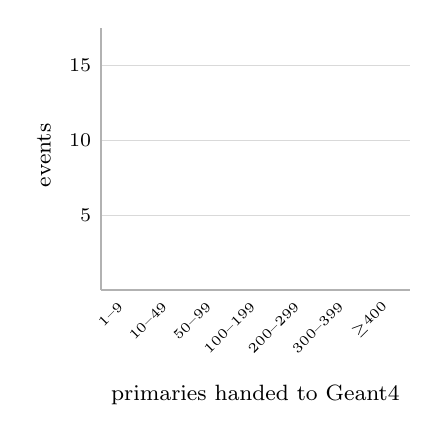
\begin{tikzpicture}[x=5.6mm, y=1.9mm, font=\scriptsize]
  \foreach \y in {5,10,15} { \draw[gray!30] (0,\y) -- (7,\y); \node[left] at (0,\y) {\y}; }
  \draw[gray!60] (0,0) -- (7,0); \draw[gray!60] (0,0) -- (0,17.5);
  \histbar{0}{4}\histbar{1}{11}\histbar{2}{15}\histbar{3}{9}\histbar{4}{5}\histbar{5}{3}\histbar{6}{3}
  \foreach \i/\l in {0/1--9,1/10--49,2/50--99,3/100--199,4/200--299,5/300--399,6/$\geq$400}
    { \node[rotate=45, anchor=east, font=\tiny] at (\i+0.6,-0.5) {\l}; }
  \node[font=\footnotesize] at (3.5,-7) {primaries handed to Geant4};
  \node[rotate=90, font=\footnotesize] at (-1.3,9) {events};
\end{tikzpicture}\hfill
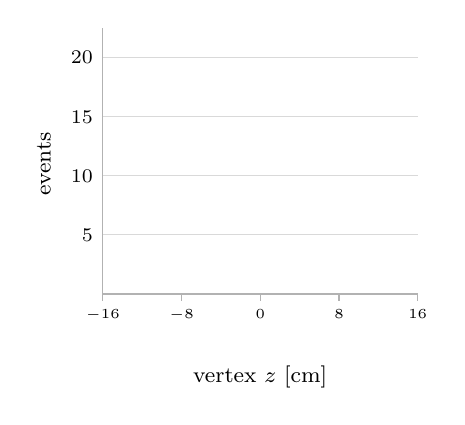
\begin{tikzpicture}[x=5.0mm, y=1.5mm, font=\scriptsize]
  \foreach \y in {5,10,15,20} { \draw[gray!30] (0,\y) -- (8,\y); \node[left] at (0,\y) {\y}; }
  \draw[gray!60] (0,0) -- (8,0); \draw[gray!60] (0,0) -- (0,22.5);
  \histbar{0}{0}\histbar{1}{2}\histbar{2}{5}\histbar{3}{20}\histbar{4}{15}\histbar{5}{7}\histbar{6}{0}\histbar{7}{1}
  \foreach \i/\l in {0/$-16$,2/$-8$,4/0,6/8,8/16} { \draw[gray!60] (\i,0) -- (\i,-0.6); \node[below, font=\tiny] at (\i,-0.5) {\l}; }
  \node[font=\footnotesize] at (4,-7) {vertex $z$ [cm]};
  \node[rotate=90, font=\footnotesize] at (-1.5,11) {events};
\end{tikzpicture}\hfill
\begin{tikzpicture}[x=5.0mm, y=2.8mm, font=\scriptsize]
  \foreach \y in {4,8,12} { \draw[gray!30] (0,\y) -- (8,\y); \node[left] at (0,\y) {\y}; }
  \draw[gray!60] (0,0) -- (8,0); \draw[gray!60] (0,0) -- (0,12.5);
  \histbar{0}{0}\histbar{1}{8}\histbar{2}{9}\histbar{3}{11}\histbar{4}{8}\histbar{5}{9}\histbar{6}{3}\histbar{7}{2}
  \foreach \i/\l in {0/$-0.4$,2/$-0.2$,4/0,6/0.2,8/0.4} { \draw[gray!60] (\i,0) -- (\i,-0.3); \node[below, font=\tiny] at (\i,-0.25) {\l}; }
  \node[font=\footnotesize] at (4,-3.8) {vertex $t$ [ns]};
  \node[rotate=90, font=\footnotesize] at (-1.5,6) {events};
\end{tikzpicture}
\caption{The 50 library events: the number of primaries handed to Geant4 (left; the bins widen to the
right), the $z$ position of the primary vertex in $4\cm$ bins (middle) and its time in $100\ps$ bins
(right). The $z$ and $t$ distributions are the luminous region of the HL-LHC beams sampled 50 times
($\sigma_z\simeq4.4\cm$, $\sigma_t\simeq160\ps$); the multiplicity distribution is the mixture of the
four process types with the MPI fluctuations of the non-diffractive class.}
\label{fig:hist}
\end{figure}

Four things to read from table~\ref{tab:stats} and figure~\ref{fig:hist}.
\begin{itemize}
\item \textbf{The library is not 50 copies of the same event.} Two events (5 and 47) hand Geant4 a single
  forward photon and leave \emph{no hit at all} in the detector; three more (6, 10, 37) leave a
  few dozen. At the other end, events 25 and 9 (633 and 614 primaries) have more primaries than the hard
  \bbbar{} signal event of the book (518). When the mixing draws 10 events for a bunch crossing, the sum is
  dominated by the two or three largest ones: in the companion chapter, event 9 (``event 2 of $\bx=0$'')
  alone carries a quarter of the in-time pileup.
\item \textbf{The process type sets the scale.} A non-diffractive event has on average 178 primaries and
  3300 tracker hits; a diffractive one 30 to 55 primaries and $\sim800$ hits. The 15 diffractive events of
  the library contribute 9\,\% of its primaries. In the pages of the mixed event they are nearly invisible;
  in the \code{PileupSummaryInfo} they count as full collisions.
\item \textbf{Most of the energy goes forward.} The hardest stable particle has $\pt<10\GeV$ in every event,
  yet the HCAL column of table~\ref{tab:events} (HF included) and the HF rows of the case-(b) log show
  hundreds of shower-library units per event in the HF: the beam remnants and the diffractive systems carry
  most of the energy at $3<|\eta|<5$. In the EB the average event deposits $12\GeV$ over $\sim8000$ hits, a
  few MeV per crystal.
\item \textbf{The vertices are spread over $\pm10\cm$ and $\pm0.3\ns$.} No library event sits at the origin;
  the one closest to it (event 12, $z=-0.03\cm$) is $0.1\ns$ away in time. The signal vertex of the book is
  at $z=0.55\cm$, $t=0$; every library event is separated from it by centimetres or by hundreds of
  picoseconds, usually both.
\end{itemize}

\begin{plainwords}[Mean, median and the two big events]
With 50 events the mean (137 primaries) is pulled up by a handful of large non-diffractive events; the
median event (75 primaries) is what one ``typically'' draws. This matters when scaling: a pileup
expectation computed from the mean per collision is right on average, but any single mixed event will
deviate from it by much more than $\sqrt{N}$, because its sum is a sum of very unequal terms. The
companion chapter's mixed event (18 collisions, 2691 primaries, mean 150) is one such draw.
\end{plainwords}

% ======================================================================================================
\FloatBarrier
\section{One library event on the detector}
\label{sec:oneevent}

{\sloppy The script draws one event of the library (\code{PUEVENT}, default 1) with the ordinary
\code{simHitAnalyzer\_cfg.py} of the SIM chapter, into \code{PU\_Phase2/pileup/<station>/}; this is case (b)
of the companion chapter. Event 1 is a non-diffractive event of 182 primaries, on the large side of the
library (rank 13 of 50), with its vertex at $z=0.03\cm$, $t=-71\ps$. On its pages every hit is coloured by
the kind of the primary it descends from, exactly as on the signal pages, and the leading primary of every
kind is followed through the layers.\par}

\begin{table}[H]
\centering\small
\caption{Event 1 of the library per station (\code{pileup/simHits.log}): \code{PSimHit}s for the tracker and
the muon system, \code{PCaloHit}s and hit cells for the calorimeters, the energy of the cells owned by
each kind of primary, and the primaries that left at least one hit in the station. HF energies in
shower-library units, HGCal energies as deposited in the active layers. Stations as in the SIM chapter:
ECAL = EB + HGCal EE, HCAL = HB + HO + HF + HGCal HSi + HSc, HGCAL = EE + HSi + HSc.}
\label{tab:stations}
\setlength{\tabcolsep}{4pt}
\begin{tabularx}{\textwidth}{lrrXr}
\toprule
station & hits & cells & energy by kind of the primary [GeV] & primaries \\
\midrule
TRK & 3439 & -- & \textcolor{sigchg}{charged hadron} 2233, \textcolor{signeu}{neutral hadron} 179, \textcolor{sigpho}{photon} 410, $e^\pm$ 19, no stored ancestor 598 (hits) & 98 of 182 \\
ECAL & 15\,156 & 4713 & \textcolor{sigchg}{9.61}, \textcolor{signeu}{2.43}, \textcolor{sigpho}{4.37}, no stored ancestor 0.43 & 99 of 182 \\
HCAL & 655 & 515 & \textcolor{sigchg}{200}, \textcolor{signeu}{10}, \textcolor{sigpho}{45}, $e^\pm$ 5 (HF in shower-library units) & 82 of 182 \\
HGCAL & 4652 & 3225 & \textcolor{sigchg}{0.41}, \textcolor{signeu}{0.11}, \textcolor{sigpho}{0.08} & 71 of 182 \\
MUON & 24 & -- & \textcolor{signeu}{neutral hadron} 12, no stored ancestor 12 (hits; all in GE0) & 1 of 182 \\
ALL & 3463 + 15\,811 & 5228 & \textcolor{sigchg}{210}, \textcolor{signeu}{12.5}, \textcolor{sigpho}{49.4}, $e^\pm$ 5, no stored ancestor 0.43 & 164 of 182 \\
\bottomrule
\end{tabularx}
\end{table}

\begin{figure}[H]
\centering
\begin{subfigure}[t]{0.49\textwidth}
  \includegraphics[width=\linewidth]{pileup/ALL/simHits_ALL_rz_run1_event1.png}
  \caption{all stations, $r$--$z$: 8691 drawn objects, 164 of the 182 primaries left hits.}
\end{subfigure}\hfill
\begin{subfigure}[t]{0.49\textwidth}
  \includegraphics[width=\linewidth]{pileup/TRK/simHits_TRK_xy_run1_event1.png}
  \caption{tracker, $x$--$y$ of the barrel: 1153 of the 3439 hits; the followed $\pi^+$ (5.8\,GeV) and $\Lambda$ (2.7\,GeV).}
\end{subfigure}\\[4pt]
\begin{subfigure}[t]{0.49\textwidth}
  \includegraphics[width=\linewidth]{pileup/TRK/simHits_TRK_rz_run1_event1.png}
  \caption{tracker, $r$--$z$: 2286 of the 3439 hits are in the endcap disks.}
\end{subfigure}\hfill
\begin{subfigure}[t]{0.49\textwidth}
  \includegraphics[width=\linewidth]{pileup/HCAL/simHits_HCAL_rz_run1_event1.png}
  \caption{hadron calorimeter, $r$--$z$: 43 HB cells with 0.04\,GeV, 161 HF cells with 260 shower-library units.}
\end{subfigure}
\caption{Library event 1 on the detector (case (b) of the companion chapter): a non-diffractive
minimum-bias collision of 182 primaries. Colour = kind of the primary the hit descends from; marker size
of a calorimeter cell = its summed energy; the grey dots are the detector elements.}
\label{fig:event1}
\end{figure}

\begin{figure}[H]
\centering
\begin{subfigure}[t]{0.49\textwidth}
  \includegraphics[width=\linewidth]{pileup/ECAL/simHits_ECAL_etaphi_run1_event1.png}
  \caption{ECAL station in $\eta$--$\phi$: 1799 EB crystals (16.3\,GeV) and 2914 HGCal EE cells (0.55\,GeV).}
\end{subfigure}\hfill
\begin{subfigure}[t]{0.49\textwidth}
  \includegraphics[width=\linewidth]{pileup/HGCAL/simHits_HGCAL_etaphi_run1_event1.png}
  \caption{HGCal station in $\eta$--$\phi$: 3225 cells, 71 primaries, no jet.}
\end{subfigure}
\caption{The calorimeters of library event 1 in $\eta$--$\phi$ seen from its vertex. The pattern is the
signature of a soft collision: hits everywhere, no cluster, the energy rising towards large $|\eta|$.}
\label{fig:event1calo}
\end{figure}

What the pages show, and what a student should take from them before seeing the mixed event:
\begin{itemize}
\item \textbf{Soft and forward.} The hardest followed primaries are a $\pi^+$ of $5.8\GeV$ at $\eta=1.83$ and a
  $\Lambda$ of $2.7\GeV$ at $\eta=0.92$; nothing in the event is above $10\GeV$. Two thirds of the tracker
  hits are in the endcap disks (figure~\ref{fig:event1}c), the EB holds $16\GeV$ spread over 1799 crystals,
  and the HF, with only 161 cells, holds most of the HCAL-station energy: the energy of a minimum-bias
  collision goes along the beam. The $x$--$y$ view of the tracker shows no bundle of tracks, only single
  curved tracks at all azimuths.
\item \textbf{A diffuse, uniform-in-$\phi$ sea.} In $\eta$--$\phi$ (figure~\ref{fig:event1calo}) the hits
  cover the whole acceptance with no structure: this is what 10 or 200 of these events stacked will look
  like, a pedestal under the signal that is flat in $\phi$ and rises with $|\eta|$.
\item \textbf{The ``no stored ancestor'' hits.} 598 tracker hits and 12 GEM hits belong to tracks whose
  ancestor \code{SimTrack} was not saved (shower secondaries below the saving thresholds, photon conversions
  far from the vertex): the grey class of the legend. They are hits like any other for the digitisers.
\item \textbf{The muon system sees almost nothing.} 24 hits, all in the innermost GEM station (GE0, up to
  $|\eta|=2.8$) and none from a muon: punch-through of a forward neutral hadron. A minimum-bias event rarely
  produces a muon that reaches the chambers.
\item \textbf{It is one event, not the average.} With 182 primaries event 1 is above the median of the
  library (75). \code{PUEVENT=25} draws the largest event, \code{PUEVENT=47} an event with no hit at all
  (section~\ref{sec:extend}).
\end{itemize}

\begin{plainwords}[What the mixing will do with this page]
Take the pages of event 1 and imagine seven of them, drawn from the library at random, stacked on top of
each other and shifted $25\ns$ earlier; then eight more with no time shift; then three more shifted
$25\ns$ later; and the signal event on top of all of them. That is the mixed event of the companion chapter.
Every hit of the library event survives the stacking unchanged except for two stamps: which collision it
came from, and which bunch crossing.
\end{plainwords}

% ======================================================================================================
\FloatBarrier
\section{How large a library must be}
\label{sec:size}

A library is consumed at a rate set by the mixing scenario: every signal event takes, on average,
$\mu\times n_{\bx}$ library events, with $n_{\bx}$ the number of bunch crossings of the window.
\begin{center}\small
\begin{tabularx}{\textwidth}{lrrlX}
\toprule
scenario & $\mu$ & window & per signal event & library size for $N$ signal events \\
\midrule
this book & 10 & $-1\ldots+1$ & 30 (18 drawn) & $30N$: 50 serves barely 2 (sequential reading) \\
in-time only, denser & 50 & $0$ & 50 & $50N$ \\
production window at $\mu=10$ & 10 & $-3\ldots+3$ & 70 & $70N$ \\
Phase-2 production & 200 & $-3\ldots+3$ & 1400 & $1400N$: $\sim0.5$\,GB read per signal event \\
\bottomrule
\end{tabularx}
\end{center}

\paragraph{Sequential and random reading.} The mixing job reads the library through a secondary source
(\code{EmbeddedRootSource}). In the exercise of this book the source reads \emph{sequentially}
(\code{sequential = True}): it starts at event 1 and reads on, so that the mixed events are the first 18 of
the library and no event is used twice; this is what makes the pages reproducible and
table~\ref{tab:events} directly comparable with the mixed event. When the library is exhausted the source
wraps around to the beginning, and the same event appears again with another event id -- harmless for a
plot, wrong for a measurement of anything. The default (\code{sequential = False}) is to jump to random
positions of the library for every signal event, so that a library much smaller than $1400N$ can serve $N$
signal events: the same library event then appears in many signal events, and the statistical
independence of the pileup between signal events is only approximate. The production accepts this: its
libraries have millions of events, and each signal event sees 1400 of them in a random combination.

\begin{plainwords}[Why reuse is acceptable]
Reusing a library event in two different signal events is like reusing the same photograph of a crowd as the
background of two different portraits. As long as the crowd is large and the portraits are unrelated,
nobody will find the correlation. It becomes a problem only when the same library event is reused within
\emph{one} signal event (the wrap-around of a too-small library), or when a library is so small that a
rare feature of one event (a $9\GeV$ particle, a punch-through in the muon chambers) appears in every mixed
event. The \code{PUEVENTS} margin of the script is there to prevent the first; the second is why the
production libraries are large.
\end{plainwords}

\paragraph{The production libraries.} The RelVal workflows of the release do exactly what this chapter
does, on a larger scale: the \code{PUDataSets} of
\path{Configuration/PyReleaseValidation/python/relval_steps.py} point the Phase-2 workflows to a minimum-bias
GEN-SIM sample made with the same fragment,
\begin{lstlisting}[style=py]
PUDataSets[ds] = {'-n': 10, '--pileup': 'AVE_200_BX_25ns', '--pileup_input': 'das:/RelValMinBias_14TeV/<release-and-conditions>/GEN-SIM'}
\end{lstlisting}
i.e.\ a dataset in DAS instead of a local file, read through its file list. The central production goes one
step further: it mixes and digitises the minimum-bias events once at $\mu=200$ into a library of
\emph{premixed} events (the \code{PREMIX} data tier, one event per signal event to come) and later adds a
single premixed event to every digitised signal event. The GEN-SIM minimum-bias library of this chapter is
the input of that premixing stage too; what changes is only where the stacking is done. The companion
chapter describes both schemes.

% ======================================================================================================
\section{Reproducing, inspecting and extending}
\label{sec:extend}

\subsection{Making the library with the script}

From an initialised \code{CMSSW\_15\_0\_5} environment:
\begin{lstlisting}[style=sh]
cd JitJetSW/Journey/test
CASES=pileup ./runPileup_mcPhase2_BBbar.sh      # generate + simulate the library (50 events) and draw event 1 into PU_Phase2/pileup/
\end{lstlisting}
With \code{CASES=pileup} the script does only what this chapter describes: it builds the plugin if needed,
runs the two \code{cmsDriver.py} steps unless the library exists (\code{REUSE=1}, the default), and draws
one event. The variables that concern the library:
\begin{center}\small
\begin{tabularx}{\textwidth}{>{\raggedright\arraybackslash}p{50mm}X}
\toprule
variable (default) & meaning \\
\midrule
\code{PUEVENTS=50} & number of events generated; must cover $\mathrm{PU}\times n_{\bx}$ per signal event with
  margin when the mixing reads sequentially \\
\code{PUSEED=20261} & random-seed base: \code{generator}, \code{VtxSmeared}, \code{g4SimHits} get
  \code{PUSEED}, $+1$, $+2$; a new seed is a new library \\
\code{PUEVENT=1} & the library event drawn alone into \code{pileup/} \\
\code{REUSE=1} & keep the existing \code{step1} / \code{step2} files whatever \code{PUEVENTS} and
  \code{PUSEED} say; \code{REUSE=0} regenerates both \\
\code{CASES=pileup} & library and its drawing only (no signal page, no mixing) \\
\code{OUTDIR=PU\_Phase2} & where everything goes \\
\code{STATIONS=TRK,ECAL}, \code{HIGHLIGHT}, \code{HIGHLIGHT\_PTMIN}, \code{PNG}, \code{PRINTHITS} & analyzer
  options of the drawing, as in \code{runSimHitAnalyzer\_mcPhase2\_BBbar.sh} \\
\code{RUN=0} & only write the \code{cmsDriver} configurations (to read or edit them) \\
\bottomrule
\end{tabularx}
\end{center}
Variations, in increasing cost:
\begin{lstlisting}[style=sh]
PUEVENT=25 CASES=pileup ./runPileup_mcPhase2_BBbar.sh                 # draw the largest event (633 primaries)
PUEVENT=47 CASES=pileup ./runPileup_mcPhase2_BBbar.sh                 # draw an event with no hit: one forward proton
PUEVENT=5 STATIONS=TRK PRINTHITS=1 CASES=pileup ./runPileup_mcPhase2_BBbar.sh   # the central-diffractive event, every primary printed
REUSE=0 PUSEED=777 CASES=pileup ./runPileup_mcPhase2_BBbar.sh         # a different library of 50 (about 5 minutes)
REUSE=0 PUEVENTS=500 CASES=pileup ./runPileup_mcPhase2_BBbar.sh       # a library large enough for PU = 50 in bx -1..1 (about 35 minutes)
\end{lstlisting}
The library is the only part of the exercise worth keeping: everything else (signal page, mixing, mixed
pages) is cheap to redo, while a 500-event library is half an hour of Geant4. This is why \code{REUSE=1}
is the default and why the script never deletes a library.

\paragraph{Practical advice.}
\begin{itemize}
\item Run from a shell with the CMSSW environment set up (\code{cmsenv} in the \code{src} directory); the
  script checks for it.
\item Run a large library in the background and keep the output; do not edit the script while it runs:
\begin{lstlisting}[style=sh]
REUSE=0 PUEVENTS=500 CASES=pileup nohup ./runPileup_mcPhase2_BBbar.sh > runPileup.lib.log 2>&1 &
tail -f PU_Phase2/step2_SIM_MinBias_out.log     # one "Begin processing" line per event
\end{lstlisting}
\item \code{REUSE=1} reuses whatever \code{step2\_SIM\_MinBias\_out.root} exists, even one made with another
  seed or size; a new seed or a larger \code{PUEVENTS} needs \code{REUSE=0}, which overwrites the library.
  Copy the old one aside first if you want to keep it.
\item The random seeds are the only thing that distinguishes two libraries made with the same options. Note
  the \code{PUSEED} of a library you keep (it is in the \code{customise\_commands} line at the top of its
  \code{\_cfg.py}).
\item Memory and disk scale linearly: 380\,kB and 3.6\,s per event, so 500 events are $190$\,MB and
  $\sim30$ minutes; 5000 events (a library for a few PU-200 signal events in the production window) are
  $1.9$\,GB and 5 hours.
\end{itemize}

\subsection{Inspecting the library}
\label{sec:inspect}

The three command-line tools and the FWLite script that produced the numbers of this chapter:
\begin{lstlisting}[style=sh]
edmDumpEventContent PU_Phase2/step2_SIM_MinBias_out.root        # the products of section 5.1
edmEventSize -v PU_Phase2/step2_SIM_MinBias_out.root            # bytes per event and per branch (uncompressed / compressed)
edmFileUtil -e PU_Phase2/step2_SIM_MinBias_out.root             # run / lumi / event numbers of the 50 events
grep -A14 "PYTHIA Event and Cross Section Statistics" PU_Phase2/step1_GEN_MinBias_out.log | tail -16   # the process table of section 3
\end{lstlisting}
\begin{lstlisting}[style=py]
# libstats.py: one line per library event with its process, multiplicities and vertex (python3 libstats.py gen.root sim.root)
import sys
from DataFormats.FWLite import Events, Handle
gen, sim = sys.argv[1], sys.argv[2]
hHep = Handle('edm::HepMCProduct'); hTrk = Handle('std::vector<SimTrack>'); hPS = Handle('std::vector<PSimHit>')
tracker = ['TrackerHitsPixelBarrelLowTof', 'TrackerHitsPixelBarrelHighTof', 'TrackerHitsPixelEndcapLowTof', 'TrackerHitsPixelEndcapHighTof',
           'TrackerHitsTIDLowTof', 'TrackerHitsTIDHighTof', 'TrackerHitsTOBLowTof', 'TrackerHitsTOBHighTof']
for e in Events(gen):
    e.getByLabel('generatorSmeared', hHep); ev = hHep.product().GetEvent()
    nstable = 0; it = ev.particles_begin()
    while it != ev.particles_end():
        if it.__deref__().status() == 1: nstable += 1
        it.__preinc__()
    v = ev.vertices_begin().__deref__().position()                       # HepMC units: mm and mm/c
    print('GEN', e.eventAuxiliary().event(), ev.signal_process_id(), nstable, '%.2f cm' % (v.z() / 10.), '%.3f ns' % (v.t() / 299.792458))
for e in Events(sim):
    e.getByLabel('g4SimHits', hTrk); trks = hTrk.product()
    nprim = sum(1 for t in trks if t.genpartIndex() > 0)                 # SimTracks with a generator link = primaries handed to Geant4
    nhits = 0
    for c in tracker:
        e.getByLabel(('g4SimHits', c), hPS); nhits += hPS.product().size()
    print('SIM', e.eventAuxiliary().event(), trks.size(), nprim, nhits)
\end{lstlisting}
Pythia8's process codes (\code{signal\_process\_id()}: 101 ND, 103/104 SD, 105 DD, 106 CD) are what
table~\ref{tab:events} calls ``proc.''; the vertex of the first HepMC vertex is the smeared primary vertex
(HepMC stores positions in mm and times in mm/$c$).

\subsection{Checks before a library is used for mixing}

A library that passes these four checks will mix correctly into a signal made with the same RelVal settings:
\begin{enumerate}
\item \code{grep -E "GlobalTag|Era\_|Geometry|VtxSmeared" step1\_GEN\_MinBias\_cfg.py}: the same global tag, era,
  geometry and vertex-smearing module as the signal's GEN configuration;
\item \code{grep initialSeed step*\_MinBias\_cfg.py}: seeds that differ from the signal's (and from the
  \code{cmsDriver.py} defaults);
\item \code{edmDumpEventContent}: \code{SimTrack}s, \code{SimVertex}s, \code{generatorSmeared} and every
  \code{PSimHit} / \code{PCaloHit} collection of section~\ref{sec:products} present;
\item \code{edmFileUtil -e}: at least $\mathrm{PU}\times n_{\bx}\times N$ events for sequential reading of
  $N$ signal events (with margin for the Poisson fluctuations), or ``enough'' for random reading.
\end{enumerate}

\subsection{Other libraries}

The recipe is the same for any scenario; only the fragment and the RelVal settings change:
\begin{itemize}
\item \textbf{Run 3}: \code{MinBias\_13p6TeV\_pythia8\_TuneCP5\_cfi} (or the 13\,TeV one) with the Run-3
  conditions, era and \code{--beamspot} of the signal, e.g.\ the settings of
  \code{runCMSDrivers\_mc2024\_BBbar\_SIM.sh}; mixing scenarios \code{AVE\_50\_BX\_25ns} or the
  \code{Run3\_Flat55To75\_PoissonOOTPU} profile;
\item \textbf{a different tune or generator}: any fragment that produces inelastic collisions works
  (\code{SoftQCD:inelastic} with another tune, EPOS, \ldots); the only requirements are the four checks
  above;
\item \textbf{heavy ions}: the pileup of a Pb--Pb run is not pileup but the underlying event of one
  collision; the RelVal workflows then use a HYDJET library (\code{RelValHydjetQ\_MinBias\_5362GeV}) with
  the same mechanism;
\item \textbf{no vertex smearing} (\code{--beamspot NoSmear}) is sometimes used for detector studies; the
  library must then be made the same way, or every pileup vertex will be off by the beam-spot width relative
  to the signal.
\end{itemize}

\subsection{Questions to test yourself}

Each can be answered from the tables of this chapter; the answers are in the footnotes.
\begin{enumerate}
\item Event 5 has 11 stable particles but only 1 primary handed to Geant4, and no hit. What are the other
  ten, and why is the one primary invisible?\footnote{Beam-pipe particles: the two surviving protons and
  the charged particles of the small central system beyond $|\eta|\simeq5.5$, dropped by the beam-pipe cut
  of \code{Generator.cc}. The one that passes is a $1.9\GeV$ photon at $\eta=4.3$: it reaches the HF but a
  photon of that energy leaves no shower-library hit there.}
\item The library has 35 non-diffractive events out of 50. Is that compatible with the cross sections?\footnote{Expected
  $0.706\times50 = 35.3$, so yes, exactly as expected; the diffractive classes (8, 4, 3 against 8.2, 5.7,
  0.8) scatter within their Poisson errors, the 3 central-diffractive events being a mild upward fluctuation.}
\item Why must the library be made with \code{--beamspot DBrealisticHLLHC}, when the mixing step itself has
  no \code{--beamspot} option?\footnote{Because the vertex position and time are set in the GEN step and
  never changed afterwards: the mixing only adds $25\ns\times\bx$. The library carries its own beam spot.}
\item If \code{PUSEED} had been left at the \code{cmsDriver.py} default, what would table~\ref{tab:events}
  look like, and which column would reveal it?\footnote{The $z$ and $t$ columns: library event $k$ would
  have the same vertex as signal event $k$ (event 1 at $z=0.55\cm$, the signal's). The multiplicity columns
  would differ from the signal (different fragment) but equally from the present table.}
\item A mixing job at $\mathrm{PU}=50$ in $\bx=-1\ldots+1$ reads this 50-event library sequentially. What
  happens?\footnote{150 events are expected per signal event; after 50 the source wraps around, and every
  library event appears three times in the mixed event, with three different event ids and possibly in
  three different bunch crossings. Regenerate with \code{PUEVENTS} of a few hundred.}
\item Which library event will dominate the in-time pileup if events 20--29 are drawn for $\bx=0$?\footnote{Event
  25: 633 primaries, 5000 \code{SimTrack}s, 12\,623 tracker hits, against 2111 primaries for the ten events
  together -- 30\,\% of the crossing from one collision.}
\item The $t$ column spans $\pm0.3\ns$. Which detectors can resolve this, and which cannot?\footnote{The MTD
  ($\sim30$--$40\ps$ per track) and the HGCal cells ($\sim50\ps$ at high energy) can; the ECAL and HCAL pulses
  and the tracker hits (apart from the MTD) integrate over much more than $0.3\ns$ and cannot.}
\end{enumerate}

% ======================================================================================================
\appendix
\section{Files of the library in \code{test/PU\_Phase2/}}
\label{app:files}

\begin{center}\small
\begin{tabularx}{\textwidth}{>{\hsize=1.2\hsize\raggedright\arraybackslash}X>{\hsize=0.8\hsize\raggedright\arraybackslash}X}
\toprule
file & content \\
\midrule
\code{step1\_GEN\_MinBias\_cfg.py} & the GEN configuration written by \code{cmsDriver.py}
  (\code{.driver.log}: the \code{cmsDriver.py} output) \\
\code{step1\_GEN\_MinBias\_out.root} (2.0\,MB) & 50 generated events: HepMC, GenParticles, gen jets and MET \\
\code{step1\_GEN\_MinBias\_out.log} & Pythia8 initialisation (cross sections, MPI tables), the process
  statistics, the \code{GenXsecAnalyzer} summary \\
\code{step2\_SIM\_MinBias\_cfg.py} & the SIM configuration \\
\code{step2\_SIM\_MinBias\_out.root} (19\,MB) & \textbf{the library}: the GEN products + SimTracks,
  SimVertices, PSimHits, PCaloHits of the 50 events \\
\code{step2\_SIM\_MinBias\_out.log} & Geant4 banner and one ``Begin processing'' line per event (the
  timestamps of section~\ref{sec:cost}) \\
\code{pileup/<station>/simHits\_<station>\_run1\_event1.pdf}, \code{\_<view>\_*.png} & event 1 drawn: one PDF
  with the three views per station, one PNG per view \\
\code{pileup/simHits.log} & the analyzer printout of event 1 (table~\ref{tab:stations}) \\
\bottomrule
\end{tabularx}
\end{center}

\section{Glossary}
\label{app:glossary}

\sloppy
\begin{description}[style=sameline,leftmargin=0pt,itemsep=2pt]
\item[pileup library] a GEN-SIM sample of minimum-bias events, simulated once and mixed many times; here
  \code{step2\_SIM\_MinBias\_out.root}.
\item[minimum bias] the inelastic collisions selected with the least possible bias; in Pythia8
  \code{SoftQCD:inelastic} = non-diffractive + single, double and central diffractive.
\item[non-diffractive, diffractive] collisions in which both protons break up (ND), or in which one (SD), both
  (DD) or neither (CD, with a central system) survive; the diffractive ones leave little in the central
  detector.
\item[inelastic cross section] $\sigin = \sigma_{\mathrm{tot}} - \sigma_{\mathrm{el}} = 78.4\mb$ at
  $14\TeV$ with the CP5 tune; the rate of pileup collisions is $\mathcal{L}\sigin$.
\item[generator fragment] the \code{\_cfi.py} file that configures the generator (process, tune, energy);
  the first argument of \code{cmsDriver.py} in a GEN step.
\item[tune (CP5)] the set of Pythia8 parameters (PDF, $\alpha_s$, MPI, colour reconnection) fitted to data;
  the same for the signal and the library.
\item[multiple-parton interactions (MPI)] several parton pairs interacting in one collision; the source of
  the large multiplicity fluctuations of non-diffractive events.
\item[stable particle] HepMC status 1: what is left after Pythia8 decayed everything with $c\tau<10\mm$.
\item[primary] a stable particle handed to Geant4 ($p>40\MeV$, not lost down the beam pipe); a
  \code{SimTrack} with \code{genpartIndex() > 0}.
\item[luminous region, beam spot] the overlap volume of the two colliding bunches, where the vertices are;
  for the HL-LHC $\sigma_z\simeq4.3\cm$, $\sigma_t\simeq190\ps$, a few $\mu$m transversely.
\item[VtxSmeared] the GEN-step module that moves every generated event to a vertex drawn from the beam
  model; \code{HLLHCEvtVtxGenerator} with database parameters for \code{--beamspot DBrealisticHLLHC}.
\item[RandomNumberGeneratorService, initialSeed] the service that owns one random engine per module; the seed
  fixes the whole sequence, and \code{cmsDriver.py} writes the same defaults into every configuration.
\item[FEVTDEBUG] the event content that keeps everything, including every SimHit collection; what a library
  needs.
\item[GEN, GEN-SIM] data tiers: generator products only; generator plus Geant4 products.
\item[SimTrack, SimVertex] the particles and vertices Geant4 kept; the \code{SimTrack} of a primary links back
  to its generator particle.
\item[PSimHit, PCaloHit] a hit in a tracker / muon / MTD sensor; an energy deposit in a calorimeter cell.
\item[sequential reading] the mixing reads the library from its first event onward (\code{sequential =
  True}); the default jumps to random positions.
\item[wrap-around] what the secondary source does when the library is exhausted: it starts again from the
  first event, so the same event appears twice in one mixed event.
\item[PREMIX] the production data tier of pileup events already mixed and digitised at the target $\mu$; made
  from a GEN-SIM minimum-bias library like this one.
\item[case (b)] in the pileup chapter: one library event drawn alone, \code{PU\_Phase2/pileup/}.
\end{description}

\end{document}
